%This is my super simple Real Analysis Homework template

\documentclass[leqno]{article}
\usepackage[utf8]{inputenc}
\usepackage[english]{babel}
\usepackage[]{amsthm} %lets us use \begin{proof}
\usepackage{amsmath}
\usepackage[]{amssymb} %gives us the character \varnothing
\usepackage{graphicx}

\title{Homework 3 -- Part I}
\author{Aline Bessa and Rao Li}
\date\today
%This information doesn't actually show up on your document unless you use the maketitle command below

\begin{document}
\maketitle %This command prints the title based on information entered above

%Section and subsection automatically number unless you put the asterisk next to them.
\section*{Question 1} Before computing principal components, let's represent the points as a matrix, with each attribute as a column and 
each row as a point:
\[
X=
  \begin{bmatrix}
    -2 & -2 \\
     0 & 0 \\
     2 & 2 \\
  -0.5 & 0.5 \\
   0.5 & -0.5 
  \end{bmatrix}
\]
The mean of both columns is zero, so the data is already mean-centered. Now let's compute the covariance matrix associated to X  
using the standard formula (denominator = $N - 1$): 
\hfill
\[
Cov=
  \begin{bmatrix}
  \frac{-2^2 + 2^2 + (-0.5)^2 + 0.5^2}{4} & \frac{-2*-2 + 2*2 + (-0.5*0.5) + 0.5*(-0.5)}{4} \\
  \frac{-2*-2 + 2*2 + (-0.5*0.5) + 0.5*(-0.5)}{4} & \frac{-2^2 + 2^2 + 0.5^2 + (-0.5)^2}{4}\\ 
  \end{bmatrix}
\]
\[
Cov=
  \begin{bmatrix}
  2.125 & 1.875 \\
  1.875 & 2.125\\ 
  \end{bmatrix}
\]
Now, let's compute the eigenvalues and eigenvectors associated to the covariance matrix:
\[
Cov - \lambda I=
  \begin{bmatrix}
  2.125 - \lambda & 1.875 \\
  1.875 & 2.125 -\lambda\\ 
  \end{bmatrix}
\]
\begin{equation*}
\begin{split}
&det(Cov - \lambda I)= (2.125 - \lambda)^2 - 1.875^2 \\
&det(Cov - \lambda I)= 4.515625 - 4.25\lambda + \lambda^2 - 3.515625 \\
&det(Cov - \lambda I)= \lambda^2 - 4.25\lambda + 1 \\
\end{split}
\end{equation*}
The eigenvalues are the solutions to $det(Cov - \lambda I) = 0$:
\begin{equation*}
\begin{split}
&\lambda^2 - 4.25\lambda + 1 = 0\\
&\lambda = \frac{4.25 \pm \sqrt{(-4.25)^2 - 4*1*1)}}{2*1}\\
&\lambda = 4\mbox{ or }\lambda = 0.25
\end{split}
\end{equation*} 
To get the first eigenvactor, using $\lambda = 4$, we do
%% \[
%%   \begin{bmatrix}
%%   2.125 - 4 & 1.875 \\
%%   1.875 & 2.125 - 4\\ 
%%   \end{bmatrix}
%% \]
\begin{gather*}
\begin{split}
&\begin{bmatrix}
    2.125 - 4 & 1.875 \\
    1.875 & 2.125 - 4\\  
\end{bmatrix} \times \begin{bmatrix}
   x_1\\
   x_2\\
\end{bmatrix} =
\begin{bmatrix}
   0\\
   0
\end{bmatrix}
\\
&\begin{bmatrix}
    -1.875 & 1.875 \\
    1.875 & -1.875\\  
\end{bmatrix} \times \begin{bmatrix}
   x_1\\
   x_2\\
\end{bmatrix} =
\begin{bmatrix}
   0\\
   0
\end{bmatrix}
\\
&\begin{bmatrix}
    -1.875x_1 + 1.875x_2 \\
    1.875x_1  -1.875x_2\\  
\end{bmatrix} =
\begin{bmatrix}
   0\\
   0\\
\end{bmatrix}
\end{split}
\end{gather*}
That is, $x_1 = x_2$ and they can be any value. For our first principal component, however, we want the $L_2$ norm of the eigenvector to be 1, i.e.,
\begin{equation*}
\begin{split}
&x_1^2 + x_2^2 = 1\\
&x_1^2 + x_1^2 = 1\\
&2x_1^2 = 1\\
&x_1 = \pm \sqrt{\frac{1}{2}}  
\end{split}
\end{equation*}
If we use $x_1 = \sqrt{\frac{1}{2}}$, our first principal component, associated to the largest eigenvalue, is
\begin{gather*}
\begin{split}
&\begin{bmatrix}
    x_1 \\
    x_2  \\
\end{bmatrix} =
\begin{bmatrix} 
   \sqrt{\frac{1}{2}}\\
   \sqrt{\frac{1}{2}}\\
\end{bmatrix}
\end{split}
\end{gather*}
As for $\lambda = 0.25$, we have our second principal component:
\begin{gather*}
\begin{split}
&\begin{bmatrix}
    2.125 - 0.25 & 1.875 \\
    1.875 & 2.125 - 0.25\\  
\end{bmatrix} \times \begin{bmatrix}
   x_1\\
   x_2\\
\end{bmatrix} =
\begin{bmatrix}
   0\\
   0
\end{bmatrix}
\\
&\begin{bmatrix}
    1.875 & 1.875 \\
    1.875 & 1.875\\  
\end{bmatrix} \times \begin{bmatrix}
   x_1\\
   x_2\\
\end{bmatrix} =
\begin{bmatrix}
   0\\
   0
\end{bmatrix}
\\
&\begin{bmatrix}
    1.875x_1 + 1.875x_2 \\
    1.875x_1 + 1.875x_2\\  
\end{bmatrix} =
\begin{bmatrix}
   0\\
   0\\
\end{bmatrix}
\end{split}
\end{gather*}
That is, $x_1 = -x_2$ and they can be any value. For our second principal component, however, we want the $L_2$ norm to be 1, i.e., 
\begin{equation*}
\begin{split}
&x_1^2 + (-x_1)^2 = 1\\
&x_1^2 + x_1^2 = 1\\
&2x_1^2 = 1\\
&x_1 = \pm \sqrt{\frac{1}{2}}  
\end{split}
\end{equation*}
If we $x_1 = \sqrt{\frac{1}{2}}$, our second principal component is:
\begin{gather*}
\begin{split}
&\begin{bmatrix}
    x_1 \\
    x_2  \\
\end{bmatrix} =
\begin{bmatrix} 
   \sqrt{\frac{1}{2}}\\
   -\sqrt{\frac{1}{2}}\\
\end{bmatrix}
\end{split}
\end{gather*}

\hfill

\section*{Question 2} To project the points onto the two principle components, we start by creating a matrix with the eigenvectors: 
\begin{gather*}
\begin{split}
E =
&\begin{bmatrix}
    \sqrt{\frac{1}{2}} & \sqrt{\frac{1}{2}} \\
    \sqrt{\frac{1}{2}} & -\sqrt{\frac{1}{2}}\\
\end{bmatrix}
\end{split}
\end{gather*}
The first and second components correspond, respectively, to the first and second lines of $E$. We now obtain the projections by 
multiplying $E$ by $X^T$:
\begin{gather*}
\begin{split}
P =
&\begin{bmatrix}
    \sqrt{\frac{1}{2}} & \sqrt{\frac{1}{2}} \\
    \sqrt{\frac{1}{2}} & -\sqrt{\frac{1}{2}}\\
\end{bmatrix} \times
\begin{bmatrix} 
   -2 & 0 & 2 & -0.5 & 0.5\\
   -2 & 0 & 2 & 0.5 & -0.5\\
\end{bmatrix} \approx
\begin{bmatrix} 
   -2.828 &  0 & 2.828 &  0 &  0\\
   0 & 0 & 0 & -0.707 & 0.707\\
\end{bmatrix}
\end{split}
\end{gather*}
So the projected points are, in the order given in Question 1: $\{(-2.828, 0), (0, 0), (-2.828, 0), (0, -0.707), (0, 0.707)\}$.

\hfill


\section*{Question 3} Let's start with the entropy criterion. Suppose $class_1 = A$ and $class_0 = B$. 
There are then 4 $A$ and 2 $B$ training examples. If we choose feature $x_1$, we have two 
subsets of examples: one to which $x_1 = 1$ ($S_l$) and one to which $x_1 = 0$ ($S_r$). The entropy for these 
subsets is 
\begin{equation*}
\begin{split}
&H(S_l) = -(\frac{3}{3}\log_2\frac{3}{3} + \frac{0}{3}\log_2\frac{0}{3}) \\
&H(S_l) = -1\log_21 = 0\\
&H(S_r) = -(\frac{2}{3}\log_2\frac{2}{3} + \frac{1}{3}\log_2\frac{1}{3}) \\
&H(S_r) = 0.918
\end{split}
\end{equation*}
Finally,
\begin{equation*}
\begin{split}
&H(after) = \frac{|S_l|H(S_l) + |S_r|H(S_r)}{|S_l| + |S_r|} = \frac{3*0 + 3*0.918}{3 + 3} = 0.459
\end{split}
\end{equation*} 
Analogously, for $x_2$ we have
\begin{equation*}
\begin{split}
&H(S_l) = -(\frac{1}{2}\log_2\frac{1}{2} + \frac{1}{2}\log_2\frac{1}{2}) \\
&H(S_l) = 1\\
&H(S_r) = -(\frac{2}{2}\log_2\frac{2}{2} + \frac{0}{2}\log_2\frac{0}{2})\\
&H(S_r) = -1\log_21 = 0\\
&H(after) = \frac{|S_l|H(S_l) + |S_r|H(S_r)}{|S_l| + |S_r|} = \frac{4*1 + 2*0}{4 + 2} = 0.667
\end{split}
\end{equation*}
Analogously, for $x_3$ we have
\begin{equation*}
\begin{split}
&H(S_l) = -(\frac{3}{4}\log_2\frac{3}{4} + \frac{1}{4}\log_2\frac{1}{4}) \\
&H(S_l) = 0.811\\
&H(S_r) = -(\frac{1}{2}\log_2\frac{1}{2} + \frac{1}{2}\log_2\frac{1}{2})\\
&H(S_r) = 1\\
&H(after) = \frac{|S_l|H(S_l) + |S_r|H(S_r)}{|S_l| + |S_r|} = \frac{4*0.811 + 2*1}{4 + 2} = 0.874
\end{split}
\end{equation*}
Finally,for $x_4$ we have
\begin{equation*}
\begin{split}
&H(S_l) = -(\frac{1}{2}\log_2\frac{1}{2} + \frac{1}{2}\log_2\frac{1}{2}) \\
&H(S_l) = 1\\
&H(S_r) = -(\frac{4}{4}\log_2\frac{4}{4} + \frac{0}{4}\log_2\frac{0}{4})\\
&H(S_r) = -1\log_21 = 0\\
&H(after) = \frac{|S_l|H(S_l) + |S_r|H(S_r)}{|S_l| + |S_r|} = \frac{4*1 + 2*0}{4 + 2} = 0.667
\end{split}
\end{equation*}
Because we want to minimize $H(after)$ to find the best split, $x_1$ will be chosen for the root.

\noindent Now let's use the Gini criterion, using $S_r$ and $S_l$ as defined above for the different $x$ features. 
For $x_1$, we have
\begin{equation*}
\begin{split}
&G(S_l) = 1 - 1^2 = 0\\
&G(S_r) = 1 - \Big(\frac{1}{3}\Big)^2 - \Big(\frac{2}{3}\Big)^2 = \frac{4}{9}\\
&G(S) = \frac{1}{2}*0 + \frac{1}{2}*\frac{4}{9} = 0.222
\end{split}
\end{equation*}
For $x_2$, we have
\begin{equation*}
\begin{split}
&G(S_l) = 1 - \Big(\frac{1}{2}\Big)^2 - \Big(\frac{1}{2}\Big)^2 = \frac{1}{2}\\
&G(S_r) = 1 - 1^2 = 0\\
&G(S) = \frac{2}{3}*\frac{1}{2} + \frac{1}{3}*0 = 0.333
\end{split}
\end{equation*}
For $x_3$, we have
\begin{equation*}
\begin{split}
&G(S_l) = 1 - \Big(\frac{3}{4}\Big)^2 - \Big(\frac{1}{4}\Big)^2 = \frac{3}{8}\\
&G(S_r) = 1 - \Big(\frac{1}{2}\Big)^2 - \Big(\frac{1}{2}\Big)^2 = \frac{1}{2}\\
&G(S) = \frac{2}{3}*\frac{3}{8} + \frac{1}{3}*\frac{1}{2} = 0.417
\end{split}
\end{equation*}
Finally, for $x_4$ we have
\begin{equation*}
\begin{split}
&G(S_l) = 1 - \Big(\frac{1}{2}\Big)^2 - \Big(\frac{1}{2}\Big)^2 = \frac{1}{2}\\
&G(S_r) = 1 - 1^2 = 0\\
&G(S) = \frac{2}{3}*\frac{1}{2} + \frac{1}{3}*0 = 0.333
\end{split}
\end{equation*}
Because the Gini criterion calculates how frequently a randomly chosen element will be wrongly identified, we want to minimize it to find the best split. 
Consequently, $x_1$ will be chosen for the root.

\noindent Now let's use the Misclassification criterion, using $S_r$ and $S_l$ as defined above for the different $x$ features. 
For $x_1$, we have
\begin{equation*}
\begin{split}
&J(S_l) = 0\\
&J(S_r) = 1\\
&J(S) = 0 + 1 = 1
\end{split}
\end{equation*}
For $x_2$, we have
\begin{equation*}
\begin{split}
&J(S_l) = 2\\
&J(S_r) = 0\\
&J(S) = 2 + 0 = 2
\end{split}
\end{equation*}
For $x_3$, we have
\begin{equation*}
\begin{split}
&J(S_l) = 1\\
&J(S_r) = 1\\
&J(S) = 1 + 1 = 2
\end{split}
\end{equation*}
Finally, for $x_4$ we have
\begin{equation*}
\begin{split}
&J(S_l) = 2\\
&J(S_r) = 0\\
&J(S) = 2 + 0 = 2
\end{split}
\end{equation*}
Because this criterion should minimize the number of points that are incorrectly classified, $x_1$ will be chosen for the root.

\hfill

\section*{Question 4} Let the discriminant functions be
\begin{equation*}
\begin{split}
&g_1(x_1, x_2) = 5x_2 + 3x_1 - 4\\
&g_2(x_1, x_2) = -3x_2 + 2x_1 - 6\\
\end{split}
\end{equation*}
We assign an example $(x_1, x_2)$ to class $C_1$ when $g_1(x_1, x_2) > g_2(x_1, x_2)$, that is
\begin{equation*}
\begin{split}
&g_1(x_1, x_2) > g_2(x_1, x_2)\\
&5x_2 + 3x_1 - 4 > -3x_2 + 2x_1 - 6\\
&8x_2 - x_1 + 2 > 0\\
&g(x_1, x_2) = 8x_2 - x_1 + 2
\end{split}
\end{equation*}
So if $g(x_1, x_2) > 0$, the example is assigned to class $C_1$; otherwise, to class $C_2$. 

\hfill

\section*{Question 5} \textbf{(a)} When there are two classes, the maximum entropy occurs when they are equaly likely, i.e., 
when \textit{half} of the examples are positive and \textit{half} are negative. The closer the proportions are to $\frac{1}{2}$, 
the higher the entropy. In the first dataset, we have that the proportions for positive and negative class are, respectively, 
$\frac{4}{9}$ and $\frac{5}{9}$. Consequently, the difference between these proportions and $\frac{1}{2}$ are the same, and can 
be calculated as
\begin{equation*}
\begin{split}
&|\frac{4}{9} - \frac{1}{2}| = \frac{|2*4 - 9*1|}{18} = \frac{1}{18} \\
\end{split}
\end{equation*}
As for the second dataset, the proportions for positive and negative class are, respectively, $\frac{1}{3}$ and $\frac{2}{3}$. 
The difference between these proportions and $\frac{1}{2}$ are the same, and can be calculates as 
\begin{equation*}
\begin{split}
&|\frac{1}{3} - \frac{1}{2}| = \frac{|2*1 - 3*1|}{6} = \frac{1}{6} \\
\end{split}
\end{equation*}
Given that the difference for the first dataset is smaller, its entropy is higher (this dataset has more 
\textit{impurity}). In other words, the entropy for the dataset with 4 positive and 
5 negative examples is higher.

\hfill

\noindent \textbf{(b)} First, let's compute the entropy of the entire dataset, namely $S$:
\begin{equation*}
\begin{split}
&Entropy(S) = -(\frac{3}{7}\log_2\frac{3}{7} + \frac{3}{7}\log_2\frac{3}{7}) \\
&Entropy(S) = 0.98522813603425152 \\
\end{split}
\end{equation*}
Now, let's compute the entropy associated to the examples where $x_1 = F$ and where $x_1 = F$.
\begin{equation*}
\begin{split}
&Entropy(S_{x_1 = F}) = -(\frac{2}{4}\log_2\frac{2}{4} + \frac{2}{4}\log_2\frac{2}{4}) \\
&Entropy(S_{x_1 = F}) = 1.0 \\
&Entropy(S_{x_1 = T}) = -(\frac{1}{3}\log_2\frac{1}{3} + \frac{2}{3}\log_2\frac{2}{3}) \\
&Entropy(S_{x_1 = T}) = 0.91829583405448956 \\
\end{split}
\end{equation*} 
Consequently, the second term of the Information Gain formula is
\begin{equation*}
\begin{split}
&Y = \sum_{v \in \{F, T\}}\frac{|S_{x_1 = v}|}{|S|}Entropy(S_{x_1 = v}) \\ 
&Y = \frac{4}{7}1.0 + \frac{3}{7}0.91829583405448956 \\
&Y = 0.9649839288804954 \\
\end{split}
\end{equation*} 
The final value for $x_1$ is thus
\begin{equation*}
\begin{split}
&Information-Gain(S) = 0.98522813603425152 - 0.9649839288804954 \\
&Information-Gain(S) = 0.020244207153756077 \\
\end{split}
\end{equation*} 

\hfill

\noindent \textbf{(c)} Using Information Gain as a criterion to choose the best initial splitting feature, we have that, for 
$x_1$, the value is 0.020244207153756077 (as calculated in \textbf{(b)}). For $x_2$, the value is
\begin{equation*}
\begin{split}
&Information-Gain(S) = Entropy(S) - \Big(\frac{4}{7}Entropy(S_{x_2 = F}) + \frac{3}{7}Entropy(S_{x_2 = T})\Big)\\
&Entropy(S_{x_2 = F}) = -(\frac{2}{4}\log_2\frac{2}{4} + \frac{2}{4}\log_2\frac{2}{4}) = 1.0\\
&Entropy(S_{x_2 = T}) = -(\frac{1}{3}\log_2\frac{1}{3} + \frac{2}{3}\log_2\frac{2}{3})) = 0.91829583405448956\\
&Information-Gain(S) = 0.98522813603425152 -\Big(\frac{4}{7}1.0 + \frac{3}{7}0.91829583405448956\Big) \\
&Information-Gain(S) = 0.020244207153756077
\end{split}
\end{equation*}
For $x_3$, the value is
\begin{equation*}
\begin{split}
&Information-Gain(S) = Entropy(S) - \Big(\frac{4}{7}Entropy(S_{x_3 = F}) + \frac{3}{7}Entropy(S_{x_3 = T})\Big)\\
&Entropy(S_{x_3 = F}) = -(\frac{2}{4}\log_2\frac{2}{4} + \frac{2}{4}\log_2\frac{2}{4}) = 1.0\\
&Entropy(S_{x_3 = T}) = -(\frac{1}{3}\log_2\frac{1}{3} + \frac{2}{3}\log_2\frac{2}{3})) = 0.91829583405448956\\
&Information-Gain(S) = 0.98522813603425152 -\Big(\frac{4}{7}1.0 + \frac{3}{7}0.91829583405448956\Big) \\
&Information-Gain(S) = 0.020244207153756077
\end{split}
\end{equation*}
The information gain is thus the same for all three attributes, so let's use $x_1$ as our root and create two sets 
$S1 = \{x^{(2)}, x^{(5)}, x^{(6)}\}$ and $S2 = \{x^{(1)}, x^{(3)}, x^{(4)}, x^{(7)}\}$, 
with examples having $x_1 = T$ and $x_1 = F$ respectively. The examples in $S1$ have mixed labels and they are not all 
equal, so we still have to split its corresponding node. Let's see which attribute gives the best information gain (either 
$x_2$ or $x_3$) here, starting with $x_2$:
\begin{equation*}
\begin{split}
&Information-Gain(S1) = Entropy(S1) - \Big(\frac{2}{3}Entropy(S1_{x_2 = T}) + \frac{1}{3}Entropy(S1_{x_2 = F})\Big)\\
&Entropy(S1) = -(\frac{1}{3}\log_2\frac{1}{3} + \frac{2}{3}\log_2\frac{2}{3}) = 0.91829583405448956 \\
&Entropy(S1_{x_2 = T}) = -(\frac{2}{2}\log_2\frac{2}{2} + \frac{0}{2}\log_2\frac{0}{2}) = 0\\
&Entropy(S1_{x_2 = F}) = -(\frac{1}{1}\log_2\frac{1}{1} + \frac{0}{1}\log_2\frac{0}{1})) = 0\\
&Information-Gain(S1) = 0.91829583405448956 -\Big(\frac{2}{3}0 + \frac{1}{3}0\Big) = 0.91829583405448956 \\
\end{split}
\end{equation*}
By using $x_2$, we get maximum information gain, so we can simply use it to split $S_1$, ending up with subsets 
$S3 = \{x^{(2)}\}$ and $S4 = \{x^{(5)}, x^{(6)}\}$. Now let's do the same analysis for $S2$, starting by calculating the information 
gain we may get with $x_2$:
\begin{equation*}
\begin{split}
&Information-Gain(S2) = Entropy(S2) - \Big(\frac{1}{4}Entropy(S2_{x_2 = T}) + \frac{3}{4}Entropy(S2_{x_2 = F})\Big)\\
&Entropy(S2) = -(\frac{2}{4}\log_2\frac{2}{4} + \frac{2}{4}\log_2\frac{2}{4}) = 1 \\
&Entropy(S2_{x_2 = T}) = -(\frac{1}{1}\log_2\frac{1}{1} + \frac{0}{1}\log_2\frac{0}{1}) = 0\\
&Entropy(S2_{x_2 = F}) = -(\frac{1}{3}\log_2\frac{1}{3} + \frac{2}{3}\log_2\frac{2}{3})) = 0.91829583405448956\\
&Information-Gain(S2) = 1 -\Big(\frac{1}{4}0 + \frac{3}{4}0.918295834054489560\Big) = 0.68872187554086717\\
\end{split}
\end{equation*}
With $x_3$ we have:
\begin{equation*}
\begin{split}
&Information-Gain(S2) = Entropy(S2) - \Big(\frac{1}{4}Entropy(S2_{x_3 = T}) + \frac{3}{4}Entropy(S2_{x_3 = F})\Big)\\
&Entropy(S2_{x_3 = T}) = -(\frac{1}{1}\log_2\frac{1}{1} + \frac{0}{1}\log_2\frac{0}{1}) = 0\\
&Entropy(S2_{x_3 = F}) = -(\frac{1}{3}\log_2\frac{1}{3} + \frac{2}{3}\log_2\frac{2}{3})) = 0.91829583405448956\\
&Information-Gain(S2) = 1 -\Big(\frac{1}{4}0 + \frac{3}{4}0.918295834054489560\Big) = 0.68872187554086717\\
\end{split}
\end{equation*}
Given that the information gain is the same with $x_2$ and $x_3$, we split $S2$ with $x_2$ and get sets 
$S5 = \{x^{(1)}, x^{(3)}, x^{(7)}\}$ and $S6 = \{x^{(4)}\}$. Set $S6$ is clean, but $S5$ is not, nor are all its 
elements equal. Consequently, we have to split it again, and the only feature left is $x_3$. By doing so, we end up 
with sets $S7 =  x^{(3)}$ and $S8 = \{x^{(1)}, x^{(7)}\}$. $S7$ is trivially clean and the elements of $S8$ are equal, so the 
algorithm stops. Figure 1 shows a graphic representation of this execution.

\begin{figure}[h!]
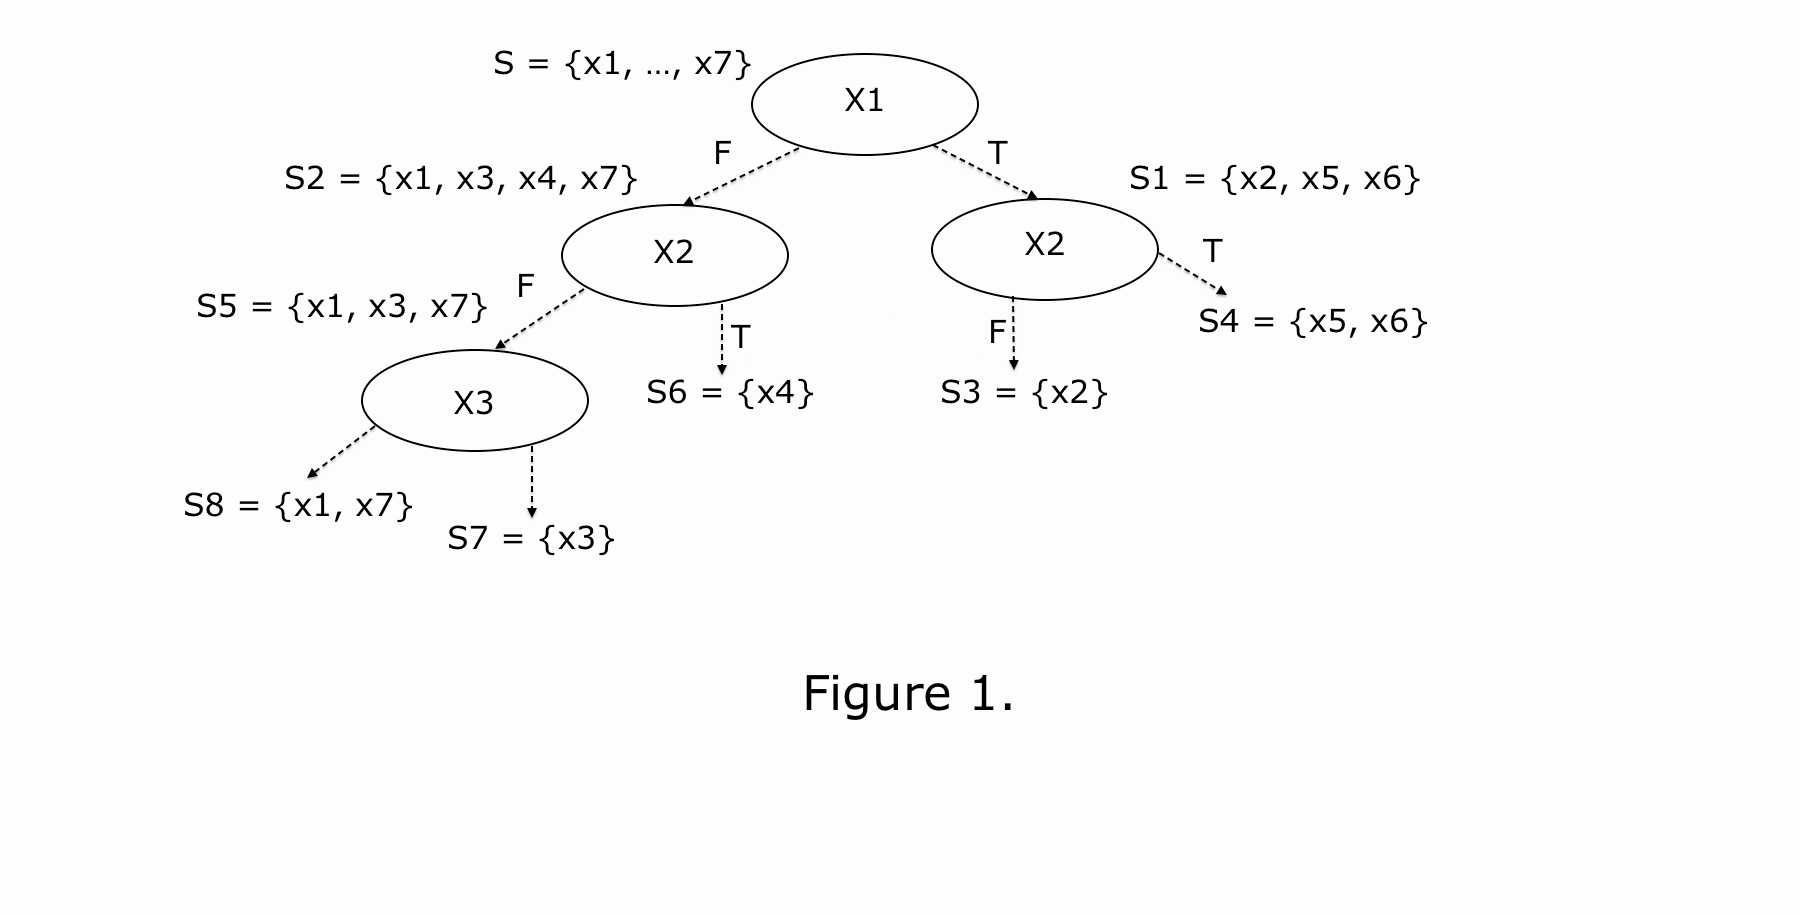
\includegraphics[width=\textwidth]{tree}  
%\caption{}
\end{figure}

\hfill

\noindent \textbf{(d)} First, let's compute $H(Y)$. 
\begin{equation*}
\begin{split}
&H(Y) = -(P[Y = +]\log_2P[Y = +] + P[Y = -]\log_2P[Y = -]) \\
&H(Y) = -(\frac{3}{7}\log_2\frac{3}{7} + \frac{4}{7}\log_2\frac{4}{7}) \\
&H(Y) = 0.98522813603425152 \\
\end{split}
\end{equation*} 
Now, let's compute $H(Y|X)$.
\begin{equation*}
\begin{split}
&H(Y|X) = \sum_xP[X = x] * \Big(\sum_y-P[Y = y| X = x]*\log_2P[Y = y| X = x]\Big) \\
%&H(Y|X) = P[X = F]*(-P[Y = +| X = F]*\log_2P[Y = +| X = F] - P[Y = -| X = F]* \log_2P[Y = -| X = F]) + P[X = T]*(-P[Y = +| X = T]*\log_2P[Y = +| X = T] - P[Y = -| X = T]*\log_2P[Y = -| X = T]) \\
&H(Y|X) = \frac{4}{7}(-\frac{1}{2}\log_2\frac{1}{2} - \frac{1}{2}\log_2\frac{1}{2}) + \frac{3}{7}(-\frac{1}{3}\log_2\frac{1}{3} - \frac{2}{3}\log_2\frac{2}{3})\\
&H(Y|X) = \frac{4}{7}*1.0 + \frac{3}{7}* 0.91829583405448956\\
&H(Y|X) = 0.9649839288804954\\
\end{split}
\end{equation*} 
Finally,
\begin{equation*}
\begin{split}
&H(Y) - H(Y|X) = 0.98522813603425152 - 0.9649839288804954 \\
&H(Y) - H(Y|X) = 0.020244207153756077
\end{split}
\end{equation*} 

\hfill

\noindent \textbf{(e)} Using the entropy formula for a dataset $S$, we have that
\begin{equation*}
\begin{split}
&Entropy(S) = -\sum_{i \in z}\frac{N_i}{N}\log_2\frac{N_i}{N}
\end{split}
\end{equation*} 
If each label is equally likely, we can write $\frac{N_i}{N} = \frac{1}{|z|}$ for any $i$. Consequently,
\begin{equation*}
\begin{split}
&Entropy(S) = -\sum_{i \in z}\frac{1}{|z|}\log_2\frac{1}{|z|}\\
&Entropy(S) = -|z|\frac{1}{|z|}\log_2\frac{1}{|z|}\\
&Entropy(S) = -\log_2\frac{1}{|z|}\\
&Entropy(S) = \log_2|z|\\
\end{split}
\end{equation*}
where $|z|$ is the number of different labels.  
\end{document}
